\chapter*{ABOUT/THIS/BOOK} 

\vspace{-0.4cm}
This book is about the code and pixels that make up the 1986 computer game \textit{Uridium}.
\textit{Uridium} was written by Andrew Braybrook, a 26 year-old programmer, on a dining-room table in Witham, Essex.
This is what it looks like.

\begin{figure}[H]
    \begin{adjustbox}{width=13cm,left}
      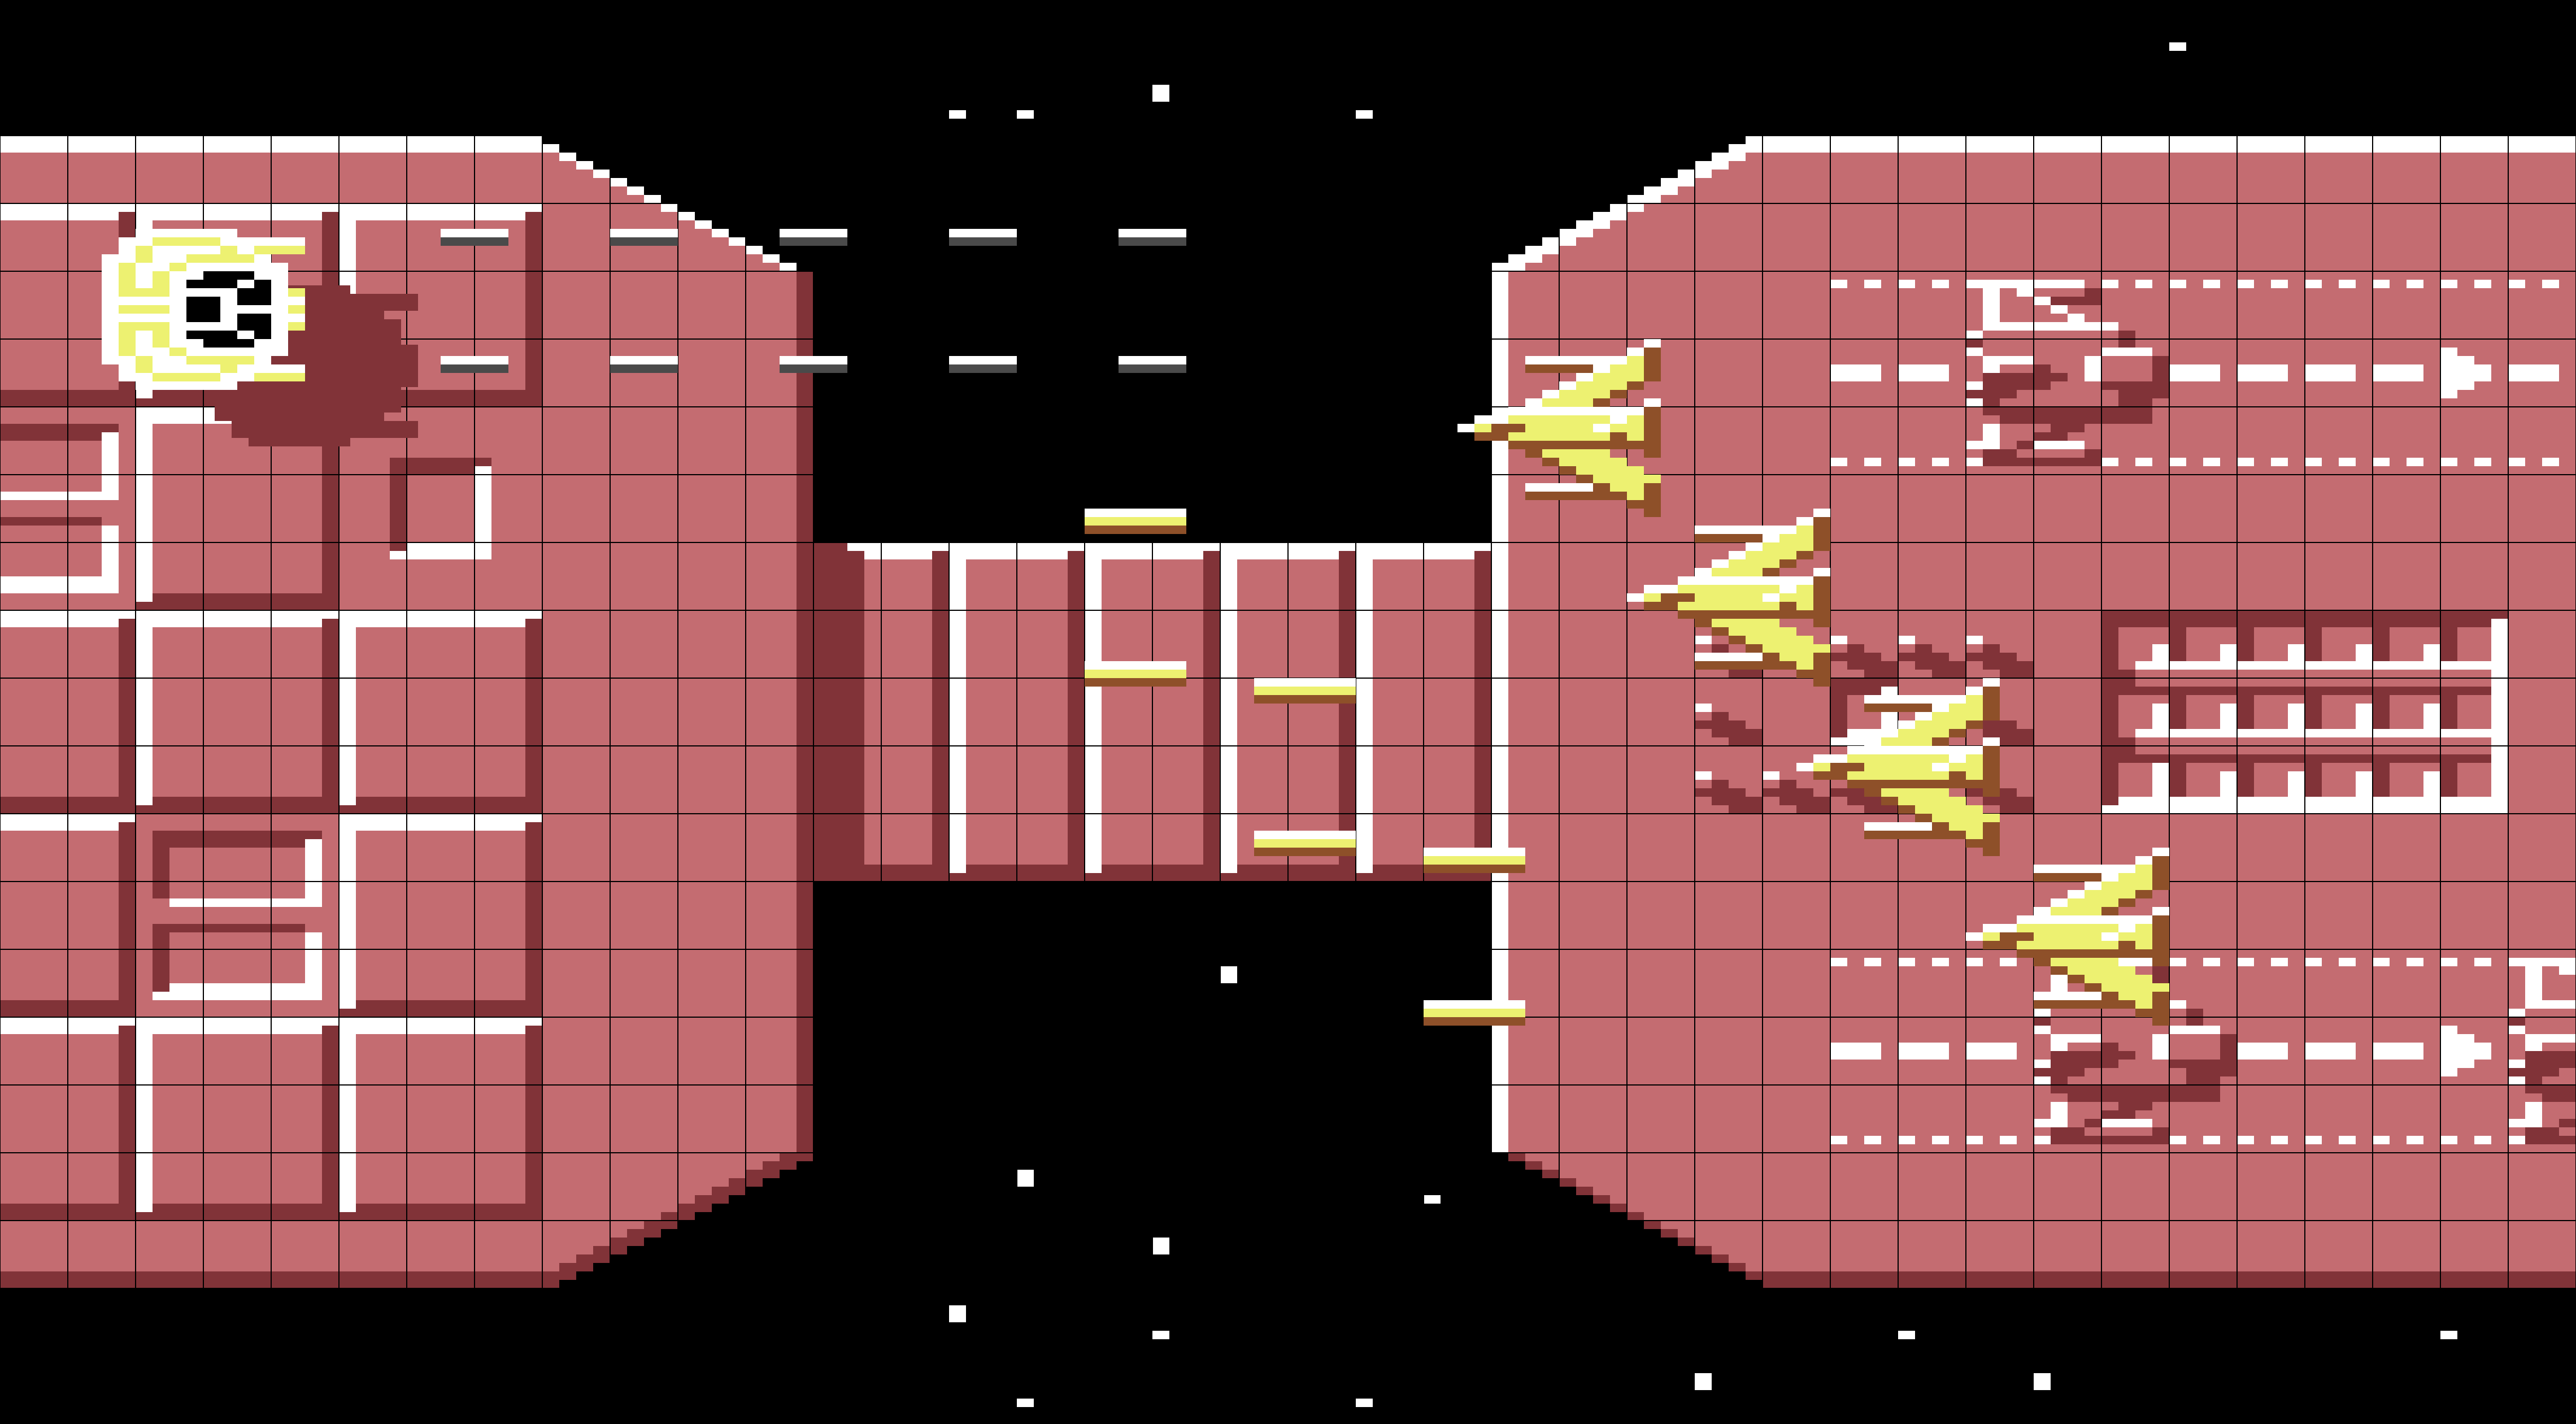
\includegraphics{src/preface/1.png}%
    \end{adjustbox}
\end{figure}
\vspace{-0.4cm}

\textit{Uridium} is from an era when a single person could program a full
videogame, in assembly language, in just a few months. Many such games were
pretty bad and are justly forgotten. \textit{Uridium} is not one of those
games. It is a slick, colourful riot, full of invention and devious technical
accomplishment. 40 years later it still deserves to be explained and enjoyed
and this book hopes to do both of those things.


Rob Hogan (\href{https://mastodon.social/@mwenge}{\textcolor{blue}{@mwenge}})\\
\the\year{} \\

\thispagestyle{empty}% Turn off page number
\clearpage
\blankpage
\vspace*{\fill}
\begin{figure}[H]
    \centering
      
\includegraphics[width=9cm]{src/cover/title_page.png}%
\end{figure}
\vspace*{\fill}
\thispagestyle{empty}% Turn off page number
\blankpage
\clearpage % Makes sure no header rule on last page

